\documentclass{article}
\usepackage{amsmath}
\usepackage{graphicx}

\title{Numerical Analysis HW 8}
\author{Michael Vu}
\date{May 1, 2017}

\begin{document}
	\maketitle
	
	\textbf{Problem 1.} For this problem and using Dr. Glunt's code, I had to change a couple lines of code. First thing I changed was setting ``iknowtheactualsolution'' to ``false'', and second change was to set function $f$ equal to $16\pi^2(x^2-x)\sin(4\pi y)-2\sin(4\pi y)$. Here is the code:
	
	
	\begin{verbatim}
			implicit none
		double precision, allocatable, dimension(:,:) :: u, unew, rhs
		double precision :: delta, f, relerr, abserr, relgot, absgot
		double precision :: actual
		logical :: iknowtheactualsolution
		integer :: iterate, n, i, j, itmax

		n = 50
		itmax = 1000000

		delta = 1.0d0/dble(n+1)
		relerr = 1.0d-7
		abserr = 1.0d-7

		iknowtheactualsolution = .false.

		allocate(u(0:n+1, 0:n+1), unew(0:n+1, 0:n+1), rhs(0:n+1, 0:n+1))
		u = 0.0d0
		unew = u 
		print*, 'Setting right hand sides'

		call setrhs(n, delta, rhs)

		open(unit = 9, file = 'Greport', status = 'replace')
		print*, 'Main loop for GS is starting'
		do iterate = 1, itmax
			call gssweep(n, u, unew, rhs, absgot, relgot)
			u = unew
			write(9,*) iterate, absgot, relgot
			
			if(absgot < abserr .and. relgot < relerr) then
				print*, 'Ha! Victory is mine at step:', iterate
				open(unit = 7, file = 'Gplot', status = 'replace')
				
				do i = 1, n 
					
					do j = 1, n
						write(7,*) delta*dble(i), delta*dble(j), u(i,j)
					end do
					
					write(7,*)
				end do
				
				if(iknowtheactualsolution) then
					call compare(n,u)
				end if
				
				close(7)
				close(9)
				print*, 'Halt'
				stop
			end if
		end do
		print*, 'Convergence not got', absgot, relgot, 'writing Gplot anyway'

		open(unit = 7, file = 'Gplot', status = 'replace')
		do i = 1, n
			
			do j = 1, n 
				write(7,*) delta*dble(i), delta*dble(j), u(i,j)
			end do
				
			write(7,*)
		end do

		if(iknowtheactualsolution) then
			call compare(n, u)
		end if

		close(7)
		close(9)

		deallocate(u, unew, rhs)
		stop
		end

		!--------subroutines and functions ---------------

		double precision function f(x, y)
		implicit none
		double precision :: x, y, pi

		pi = 3.14159265359d0

		f = 16.0d0*pi**2 *(x**2 -x) *sin(4.0d0*pi*y)-2.0d0*sin(4.0d0*pi*y)

		return
		end

		subroutine setrhs(n, delta, rhs)
		implicit none
		integer :: n, i, j
		double precision :: delta, f, rhs(0:n+1, 0:n+1)

		do i = 1, n 
			do j = 1, n 
				rhs(i,j) = delta**2 * f(delta*dble(i), delta*dble(j))
			end do
		end do

		return 
		end

		subroutine gssweep(n, u, unew, rhs, absgot, relgot)
		implicit none
		integer :: n, i, j
		double precision :: absgot, relgot, diffa, diffr
		double precision :: u(0:n+1, 0:n+1), unew(0:n+1, 0:n+1), rhs(0:n+1, 0:n+1)
		double precision :: bot

		absgot = 0.0d0 
		relgot = 0.0d0 

		do i = 1, n 
			do j = 1, n 
				unew(i,j) = (rhs(i,j) -u(i-1,j) -u(i+1,j) -u(i,j-1) -u(i,j+1)) /(-4.0d0)
				
				diffa = abs(u(i,j) - unew(i,j))
				if(diffa > absgot) then 
					absgot = diffa
				end if
				
				bot = abs(u(i,j))
				if(bot == 0.0d0) then
					bot = 1.0d0 
				end if
				
				diffr = diffa/bot 
				if(diffr > relgot) then
					relgot = diffr 
				end if 
				
				u(i,j) = unew(i,j)
			end do 
		end do

		return
		end

		double precision function actual(x,y)
		implicit none 
		double precision :: x, y 

		actual = x*y * (1.0d0 - x) * (1.0d0 - y)

		return
		end 

		subroutine compare(n,u)
		implicit none 
		integer :: n, i, j 
		double precision :: u(0:n+1, 0:n+1), x, y, delta, actual 
		double precision :: diff, worstabs, worstrel, bot 

		delta = 1.0d0/dble(n+1)
		worstabs = 0.0d0 
		worstrel = 0.0d0 

		print*, '-----------------------------------------------'
		write(9,*) '-----------------------------------------------'
		do i = 1,n 
			do j = 1,n 
				x = dble(i)*delta 
				y = dble(j)*delta 
				diff = abs(u(i,j) - actual(x,y))
				if(diff > worstabs) then 
					worstabs = diff 
				end if
				
				bot = abs(u(i,j))
				if(bot == 0.0d0) then
					bot = 1.0d0 
				end if 
				
				diff = diff/bot 
				if(diff > worstrel) then 
					worstrel = diff 
				end if 
				
			end do
		end do 

		write(9,*) 'Max Uij-actual(xi,yj)=', worstabs
		write(9,*) 'Max relerror=', worstrel
		write(*,*) 'Max Uij-actual(xi,yj)=', worstabs
		write(*,*) 'Max relerror=', worstrel

		print*, '--------------------------------------------------'
		write(9,*) '----------------------------------------------------'

		return 
		end 

	\end{verbatim}
	
	I then ran the output file Gplot in gnuplot and here are a few shots of the graph:
	
	\begin{figure}[h]
		\centering
			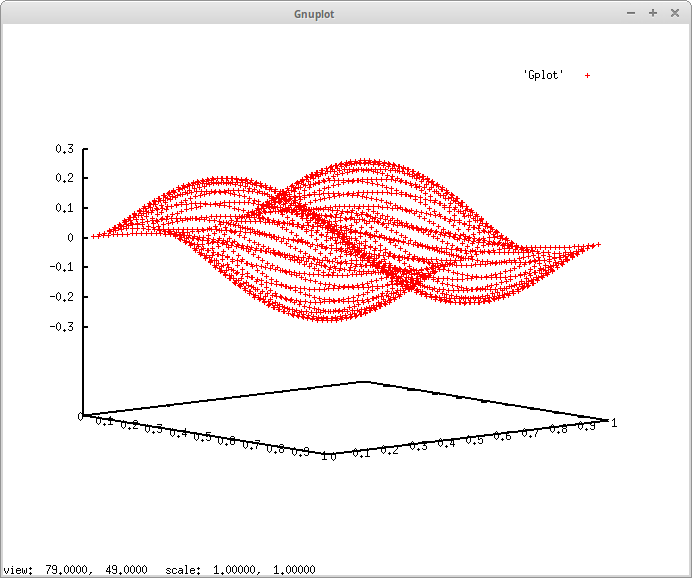
\includegraphics[width=0.75\textwidth]{C:/Users/Michael/Dropbox/NumericalAnalysis/HW08_FINAL/pr1graphs/pr1_1.png}
		\label{fig:pr1_1}
	\end{figure}
		
	\begin{center}
		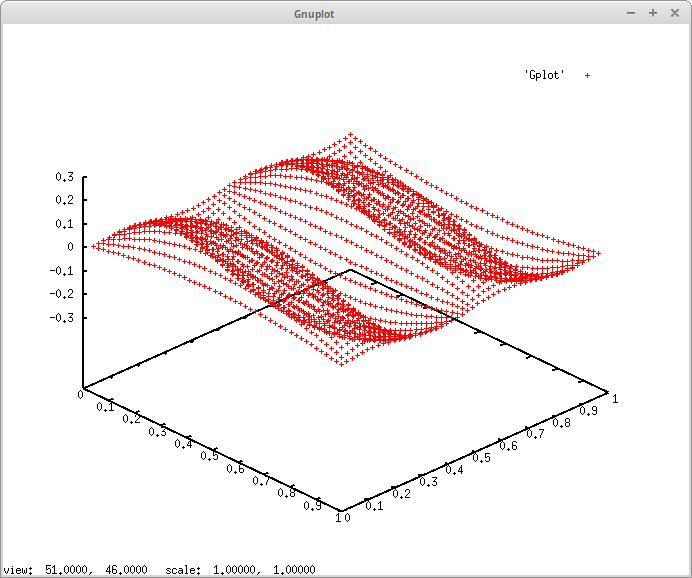
\includegraphics[width=0.75\textwidth]{C:/Users/Michael/Dropbox/NumericalAnalysis/HW08_FINAL/pr1graphs/pr1_2.png}
	\end{center}
	
	\begin{center}
		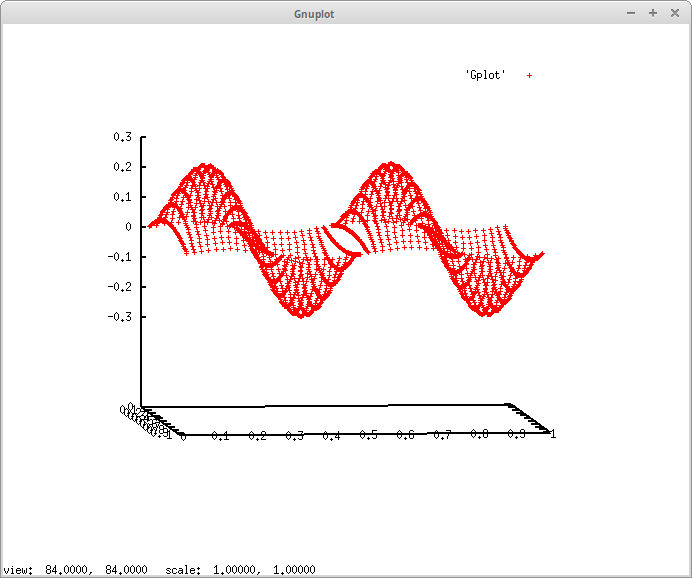
\includegraphics[width=0.75\textwidth]{C:/Users/Michael/Dropbox/NumericalAnalysis/HW08_FINAL/pr1graphs/pr1_3.png}
	\end{center}
	
	\newpage
	\textbf{Problem 2.} To solve the problem $\frac{\partial^2u}{\partial x^2}+\frac{\partial^2u}{\partial y^2}=u+f(x,y)$, I did some basic algebra to isolate $f(x,y)$, and then using the descretionization of the second derivatives as described in our lectures, we have:
	
	\begin{equation*}
		\frac{u_{i-1,j}-2u_{i,j}+u_{i+1,j}}{\Delta^2}+\frac{u_{i,j-1}-2u_{i,j}+u_{i,j+1}}{\Delta^2}-u_{i,j}=f_{i,j}\\
		
		u_{i-1,j}-2u_{i,j}+u_{i+1,j}+u_{i,j-1}-2u{i,j}+u_{i,j+1}-\Delta^2u_{i,j}=\Delta^2f_{i,j}\\
		
		(-4-\Delta^2)u_{i,j}=\Delta^2f_{i,j}-u_{i-1,j}-u_{i+1,j}-u_{i,j-1}-u_{i,j+1}\\
		
		u_{i,j}=\frac{\Delta^2f_{i,j}-u_{i-1,j}-u_{i+1,j}-u_{i,j-1}-u_{i,j+1}}{-4-\Delta^2}
	\end{equation*}
	
	\bigskip
	Using our new $u_{i,j}$, I would then change the code in the program so that $unew_{i,j}=\frac{\Delta^2f_{i,j}-u_{i-1,j}-u_{i+1,j}-u_{i,j-1}-u_{i,j+1}}{-4-\Delta^2}$. Here are the snips of sections of code I changed from the previous problem's code:
	
	
	\begin{verbatim}
		double precision function f(x, y)
			implicit none
			double precision :: x, y

			f = cos(6.0d0*(x**2 + y**2))

			return
		end
		
		subroutine gssweep(n, u, unew, rhs, absgot, relgot)
			implicit none
			integer :: n, i, j
			double precision :: absgot, relgot, diffa, diffr
			double precision :: u(0:n+1, 0:n+1), unew(0:n+1, 0:n+1), rhs(0:n+1, 0:n+1)
			double precision :: bot

			absgot = 0.0d0 
			relgot = 0.0d0 

			do i = 1, n 
				do j = 1, n 
					unew(i,j) = (rhs(i,j) -u(i-1,j) -u(i+1,j) -u(i,j-1) -u(i,j+1)) /(-4.0d0-(1.0d0/dble(n+1))**2)
					
					diffa = abs(u(i,j) - unew(i,j))
					if(diffa > absgot) then 
						absgot = diffa
					end if
					
					bot = abs(u(i,j))
					if(bot == 0.0d0) then
						bot = 1.0d0 
					end if
					
					diffr = diffa/bot 
					if(diffr > relgot) then
						relgot = diffr 
					end if 
					
					u(i,j) = unew(i,j)
				end do 
			end do

			return
		end
	\end{verbatim}
	
	I then ran the output file Gplot through gnuplot, and here are a few pictures of the graph:
		
	\begin{center}
		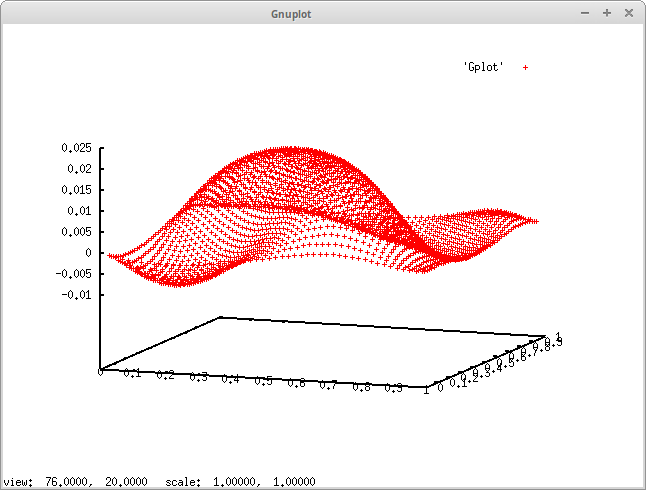
\includegraphics[width=0.70\textwidth]{C:/Users/Michael/Dropbox/NumericalAnalysis/HW08_FINAL/pr3graphs/pr3_1.png}
	\end{center}
		
	\begin{center}
		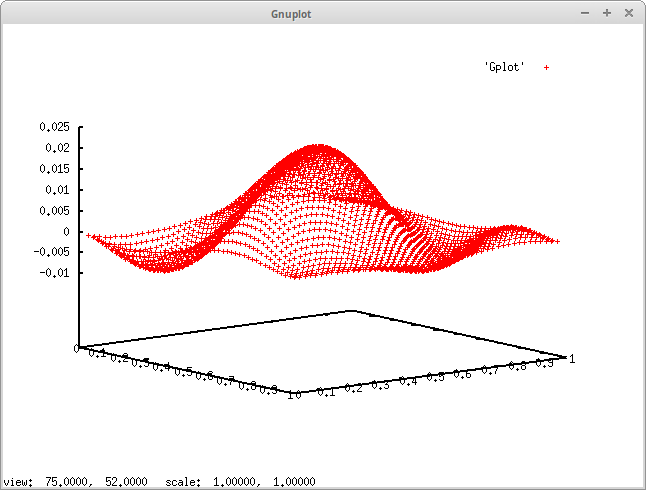
\includegraphics[width=0.75\textwidth]{C:/Users/Michael/Dropbox/NumericalAnalysis/HW08_FINAL/pr3graphs/pr3_2.png}
	\end{center}
		
	\begin{center}
		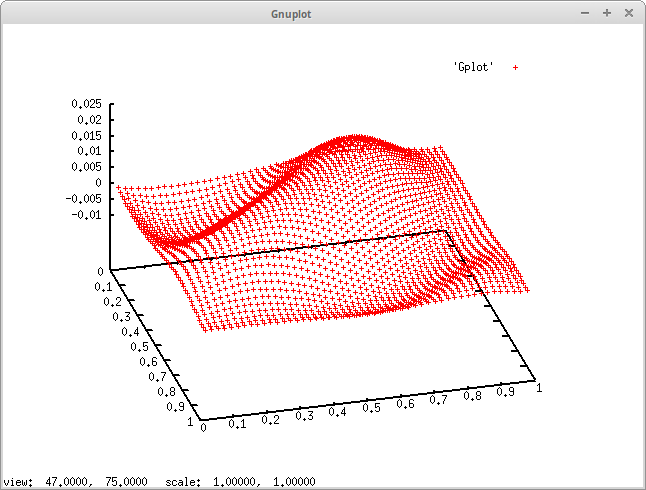
\includegraphics[width=0.75\textwidth]{C:/Users/Michael/Dropbox/NumericalAnalysis/HW08_FINAL/pr3graphs/pr3_3.png}
	\end{center}


\end{document}